\documentclass[11pt]{article}
\usepackage{amsmath,amstext,amsfonts,amssymb,amsthm,epsfig,epstopdf,array}
\usepackage[margin=1in]{geometry}
\usepackage[dvipsnames]{xcolor}
\usepackage{graphicx}
\usepackage{times}

\theoremstyle{plain}
\newtheorem{thm}{Theorem}[section]
\newtheorem{lem}[thm]{Lemma}
\newtheorem{prop}[thm]{Proposition}
\newtheorem{cor}[thm]{Corollary}
\newtheorem{defn}[thm]{Definition}
\newtheorem{claim}[thm]{Claim}

\theoremstyle{definition}
\newtheorem{con}{Conjecture}[section]
\newtheorem{exa}{Example}[section]
\newtheorem*{sol}{Solution}
\newtheorem{cdef}{Definition}[section]


\theoremstyle{remark}
\newtheorem{rem}{\textbf{Remark}}
\newtheorem*{note}{\color{blue}\textbf{Note}}
\usepackage{qtree}


\usepackage{hyperref}

\usepackage[nameinlink,noabbrev,capitalize]{cleveref} 
\crefalias{subequation}{equation}
\crefalias{thm}{theorem}


% to make cleveref print ``Lemma'' for lemma
\let\oldlemma\lem
\renewcommand{\lem}{%
  \crefalias{thm}{lem}% Theorem counter now looks like Lemma
  \oldlemma}
\Crefname{lem}{Lemma}{Lemmas}

% to make cleveref print ``Definition for definition
\let\olddefn\defn
\renewcommand{\defn}{%
  \crefalias{thm}{defn}% Theorem counter now looks like Definition
  \olddefn}
\Crefname{defn}{Definition}{Definitions}

% to make cleveref print ``Remark for remark
\let\oldrem\rem
\renewcommand{\rem}{%
  \crefalias{thm}{rem}% Theorem counter now looks like Remark
  \oldrem}
\Crefname{rem}{Remark}{Remarks}

% to make cleveref print ``Corollary for corollary
\let\oldcor\cor
\renewcommand{\cor}{%
  \crefalias{thm}{cor}% Theorem counter now looks like Corollary
  \oldcor}
\Crefname{cor}{Corollary}{Corollaries}

% to make cleveref print ``Claim for claim
\let\oldclaim\claim
\renewcommand{\claim}{%
  \crefalias{thm}{claim}% Theorem counter now looks like Claim
  \oldclaim}
\Crefname{claim}{Claim}{Claims}

% to make cleveref print ``Proposition for prop
\let\oldprop\prop
\renewcommand{\prop}{%
  \crefalias{thm}{prop}% Theorem counter now looks like Prop
  \oldprop}
\Crefname{prop}{Proposition}{Propositions}

% to make cleveref print ``Conjecture for conj
\let\oldcon\con
\renewcommand{\con}{%
  \crefalias{thm}{con}% Theorem counter now looks like Con
  \oldcon}
\Crefname{con}{Conjecture}{Conjectures}

\bibliographystyle{plain}

% BK: Editing commands requiring color package
\newcommand{\add}[1]{\textcolor{blue}{#1}}
\newcommand{\delete}[1]{\textcolor{red}{#1}}
\definecolor{darkgrn}{rgb}{0, 0.75, 0}
\newcommand{\modified}[1]{\textcolor{darkgrn}{#1}}

\newcommand{\p}{\phantom{-}}


\usepackage{hyperref}
\hypersetup{
    colorlinks=true,
    linkcolor=blue,
    filecolor=magenta,      
    urlcolor=cyan,
}
 
\urlstyle{same}

\begin{document}
\begin{center}
\textbf{To What Degree Can We Use Degree?} % Theory Blog}
\end{center}

\section{Introduction}
The \emph{degree} of a function $f$ defined on a set $\Omega$
%and $f\left(\Omega\right)$
is an extension of the \href{https://en.wikipedia.org/wiki/Winding_number}{winding number},
which counts the number of times a closed curve travels counterclockwise around a given point.
Intuitively, the degree counts the number of times $f$, in some sense, ``wraps'' $\Omega$ around a point in $f\left(\Omega\right)$.   
So what additional information does the degree give, and why would you care about it?
The degree was developed as a way to measure, or keep careful count of, the number of solutions to a system of nonlinear equations.
By ``careful'' we mean consistent with respect to some types of perturbation of the system.
Degree theory, as we shall see shortly, provides some very nice tools for verifying the existence of solutions to nonlinear systems of equations. 

\medskip
We will keep this conversation light, general and mostly geared towards imparting an intuition concerning what information the degree imparts and in what ways an application oriented person not necessarily familiar with higher level mathematics could use the degree to their general advantage. For the curious mathematician wishing for a more in depth and general derivation and application there are many summaries, blogs, lecture notes, thesis's (check \href{http://jultika.oulu.fi/files/isbn9789514284878.pdf}{this one} out for instance) etc. awaiting you on the web (Google is always your friend). Here we will not give many proofs, but the ones we do will be, hopefully, well explained and as low level as I can make them. If that is agreeable to you then let us proceed. 

\medskip
To keep the discussion simple, %In this post
we will concern ourselves with degrees of continuous functions over bounded, "nice" manifolds. In particular we will narrow our focus at the moment to smooth functions over bounded regions in $\mathbb{R}^n$. With that in mind let us define the following: 
\begin{subequations}\label{eq:Vars}
\begin{align}
& \Omega\subset\mathbb{R}^n \text{ open and bounded }\\
& f:\bar{\Omega}\rightarrow \mathbb{R}^n \text{ smooth } \\
& y\in f\left(\bar{\Omega}\right)\setminus f\left(\partial\Omega\right) \text{ a "regular value" with respect to $f$}
\end{align}
\end{subequations}
In other words $y$ is in the range of $f$ over the closure of $\Omega$ but not in the image of $f$ over the boundary of $\Omega$, and if $x\in\Omega$ such that $f(x)=y$ then $x$ is \emph{not} a \href{https://en.wikipedia.org/wiki/Critical_point_(mathematics)}{critical point} of $f$. For example in the following figure $F:\mathbb{R}^2\rightarrow\mathbb{R}^2$ with $\Omega$ the filled circle and $F(\Omega)$ the filled triangle. In this simple example $F$ maps the boundary of the circle to the boundary of the triangle, and hence the degree is not defined for any point along the boundary of the triangle. Additionally notice that the points along the red and green curves in the circle corresponding to the red and green curves in the triangle represent critical points for which the degree is not defined. However, every other point in the interior of the triangle is fair game if we assume a smooth map everywhere else.
\begin{center}
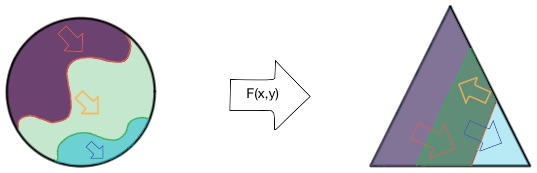
\includegraphics[scale=0.4]{Figures/R2Ex}
\end{center}


\begin{cdef}[Degree] \ \\
$$\operatorname{deg}\left(f,\Omega,y\right)=\sum\limits_{x\in f^{-1}(y)}\operatorname{sign}\left(J_f(x)\right)$$
\end{cdef}

Where $\operatorname{sign}\left(J_f(x)\right)$ denotes the sign of the \href{https://en.wikipedia.org/wiki/Jacobian_matrix_and_determinant}{Jacobian} of $f$ at $x$, i.e.:

\[\operatorname{sign}\left(J_f(x)\right)=   \left\{
\begin{array}{ll}
      -1   & \mbox{if } J_f(x)< 0, \\
      \p 0 & \mbox{if } J_f(x)= 0,~\mbox{ and } \\
      \p 1 & \mbox{if } J_f(x)> 0. \\
\end{array} 
\right. \]

By restricting ourselves to the parameters of \eqref{eq:Vars} we ensure that $\operatorname{sign}\left(J_f(x)\right)$ exists for each $x\in f^{-1}(y)$.
Thus to guarantee $\sum\limits_{x\in f^{-1}(y)}\operatorname{sign}\left(J_f(x)\right)$ exists, we need only show that the sum is finite, i.e., that  $f^{-1}(y)=\{x\in\Omega|f(x)=y\}$ is finite.
We will show this result now as it helps to illustrate the concept of degree. 

\begin{prop} \label{finite}
Given $\Omega$, $f$ and $y$ as defined in \eqref{eq:Vars}, $f^{-1}(y)=\{x\in\Omega|f(x)=y\}$ is finite. 
\begin{proof}
We will show this using a proof by contradiction which will utilize some basic results from analysis and the application of the Inverse Function Theorem. \\

Assume $f^{-1}(y)$ defines an infinite set. Then since $f^{-1}(y)\subseteq\Omega\subset\mathbb{R}^n$ and $\Omega$ is bounded we have that there must exist a limit point of $f^{-1}(y)$, i.e. $\exists \alpha\in\mathbb{R}^n$ and infinite sequence $\{x_i\}\subset f^{-1}(y)$ such that $\lim\limits_{i\rightarrow\infty}x_i=\alpha$. \\

Now since $\bar{\Omega}$ is a closed and bounded subset of $\mathbb{R}^n$ we have that it is a compact set. By \eqref{eq:Vars} we have that $x_i\in\Omega \ \forall i$, and thus it follows that $\alpha\in\bar{\Omega}$ ($\bar{\Omega}$ is compact and hence contains all of it's limit points). Since $f$ is smooth we have that $y=\lim\limits_{i\rightarrow\infty}f(x_i)=f\left(\lim\limits_{i\rightarrow\infty}x_i\right)=f(\alpha)$.\\

Since $f(\alpha)=y$, $\alpha\in\bar{\Omega}$ and by our assumptions in \eqref{eq:Vars} we have that:
\begin{itemize}
\item $\alpha\in f^{-1}(y)$
\item $\alpha\in \Omega$
\item $\alpha$ is not a critical point
\end{itemize}

Since $\alpha$ is not a critical point, $f$ is smooth, and $\Omega$ is open, we have by the \href{https://en.wikipedia.org/wiki/Inverse_function_theorem}{Inverse Function Theorem} that there exists a neighborhood, $N_{\alpha}$, of $\alpha$ lying in $\Omega$ such that $f$ is invertible over $f(N_{\alpha})$.
However, since $f(\alpha)=y$ this implies that there does not exist $x\in N_{\alpha}\setminus\{\alpha\}$ such that $f(x)=y$.
Put another way, we have that $N_{\alpha}\bigcap f^{-1}(y)=\alpha$. This is of course a contradiction as $\alpha$ is a limit point of $f^{-1}(y)$ (i.e., every neighborhood of $\alpha$ contains infinitely many points of $f^{-1}(y)$).
The proposition now follows.
\end{proof}
\end{prop}

Great, \cref{finite} guarantees that the degree under the restrictions in \eqref{eq:Vars} will always exist. Now, how can this benefit us?
Note that by the definition of the degree we can conclude readily that a solution to $f(x)=y \ \text{ for } x\in\Omega$ exists if $\operatorname{deg}\left(f,\Omega,y\right)\neq 0$. Let's illustrate this with a simple example. Consider the following simple graph of what we will assume to be a smooth function $f:\mathbb{R}\rightarrow\mathbb{R}$. 
\begin{center}
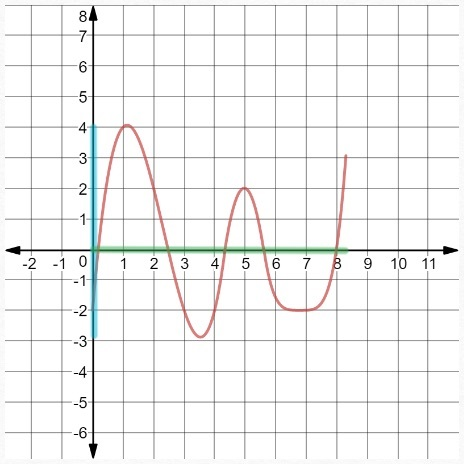
\includegraphics[]{Figures/Curveb}
\end{center}

Here we can define $\color{OliveGreen}{\Omega\approx (0,8.3)}$, giving us $\color{Cyan}{f(\Omega)\approx (-2.8,4.1)}$.
Observe that certainly $y=0$ is a regular value of $f$ over $\Omega$ which does not lie on the boundary of $f(\Omega)$.
Thus we can compute $\operatorname{deg}\left(f,\Omega,y\right)$ to be $1+(-1)+1+(-1)+1=1$. Intuitively $f$ takes the set $\Omega$, stretches it out and starts laying it down on $\Omega$ the way you would lay a long sheet down on a short surface (folding back and forth so it fits on the surface). Any regular value lying between the boundary points has the beginning of the sheet below it and the end above it, so $f$ lays over it at least 1 time (something very reminiscent of the intermediate value theorem.)
This might seem trivial, and it is, but when $\Omega$ and $f$ are not so nice the degree becomes an invaluable tool with the help of some well meaning theorems.

  

%\newpage

\section{Theory for Applications}

Alright, so what's the use of all this stuff about degree any way? For some of you, it might all seem like a waste of time because, by definition, in order to calculate the degree we must have knowledge of solutions to the very equation we are trying to verify solutions to. Despair not, however, for the following theorem will put your concerns to rest. 
This theorem is quoted directly from \cite{OrChCh2006}, which we will direct the reader to for details of a proof if interested. 

\begin{thm} \label{DegThm}
Let $\Omega\subset\mathbb{R}^b$ be an open bounded subset and $f:\bar{\Omega}\rightarrow\mathbb{R}^b$ be a continuous mapping. If $p\not\in f\left(\partial\Omega\right)$, then there exists an integer $\operatorname{deg}\left(f, \Omega,p\right)$ satisfying the following properties:
\begin{enumerate}
\item (Normality) $\operatorname{deg}\left(I, \Omega,p\right)=1$ if and only if $p\in\Omega$, where $I$ denotes the identity mapping;
\item (Solvability) If $\operatorname{deg}\left(f, \Omega,p\right)\not= 0$, then $f(x)=p$ has a solution in $\Omega$;
\item (Homotopy) If $f_t(x):[0,1]\times\bar{\Omega}\rightarrow\mathbb{R}^N$ is continuous and $p\not\in \bigcup\limits_{t\in[0,1]}f_t\left(\partial\Omega\right)$, then $\operatorname{deg}\left(f, \Omega,p\right)$ does not depend on $t\in[0,1]$. 
\item (Additivity) Suppose that $\Omega_1, \Omega_2$ are two disjoint open subsets of $\Omega$ and $p\not\in f\left(\bar{\Omega}-\Omega_1\cup\Omega_2\right)$. Then $\operatorname{deg}\left(f, \Omega,p\right)=\operatorname{deg}\left(f, \Omega_1,p\right)+\operatorname{deg}\left(f, \Omega_2,p\right)$;
\item $\operatorname{deg}\left(f, \Omega,p\right)$ is a constant on any connected component of $\mathbb{R}^n\setminus f(\partial\Omega)$. 
\end{enumerate}
\end{thm}

What \cref{DegThm} has done to our assumptions in \eqref{eq:Vars} is relax some of the restrictions, by only requiring the function to be continuous and the point in consideration not necessarily regular in all cases.
One nice advantage \cref{DegThm} has given us is seen in the homotopy invariance property or Result 3 of \cref{DegThm}.
What this allows us to do is equate the verification of solutions to one system with solutions to another, potentially much simpler system.
For instance, Frommer, Hoxha, and Lang were able to develop a test involving interval arithmetic to prove existence of zeros of functions using interval arithmetic, which depends on the homotopy invariance property of the degree \cite{FrHoLa2007}.
Of course there is a wide range of theory concerning the computation of the degree outside of utilizing just the properties found in \cref{DegThm}, which I invite you to explore. 
Here are some quick suggestions to take a look at: \cite{MoVrYa2002}, \cite{OnTh2006}, and of course the book from which we took the theorem \cite{OrChCh2006}. Additionally, keep an eye out for my own collaborative research with \href{https://dvij.github.io/}{Dr. Dvijotham}, \href{http://www.math.wsu.edu/math/faculty/bkrishna/}{Dr. Krishnamoorthy} where we take full advantage of the homotopy invariance property of  \cref{DegThm} to construct optimization based techniques for calculating robustness of solutions to systems of quadratic equations. Check \href{http://www.benrapone.com/}{my own website} to see more about myself, and new blog posts about our research on this topic once completed.

  
\bibliography{degree}

\end{document}
